\documentclass[12pt,letterpaper]{article}

\usepackage{graphicx,wrapfig,colordvi,color,citesort,times,array,subfigure,floatflt,makeidx,framed,boxedminipage,url,hyperref}

\graphicspath{{images/}}
\definecolor{UglyBrown}{rgb}{0.7,0.4,0.1} 
\newcommand{\newtext}[1]{\textcolor{UglyBrown}{#1}}

\newcommand{\contributors}{
Thomas Parker\\
Devon Jones\\
James Dempsey\\
Aaron Divinsky\\
Tir Gwaith (Andrew McDougall)\\
Frank Kliewe\\
Eddy Anthony\\
Thomas Clegg\\
Paul W. King\\
Paul Grosse\\
Terry FitzSimons\\
Chris Chandler\\
Martijn Verburg\\
Connor Petty\\
}
\newcommand{\lastupdate}{June 27, 2008}
\newcommand{\versionEOS}{0.60}
\newcommand{\docnumEOS}{2.0}
\newcommand{\lastversionEOS}{0.51}
\newcommand{\pcgenversEOS}{5.16}
\newcommand{\systemEOS}{Rules Persistence System}

\makeindex

\hoffset=-0.6in
\voffset=-0.6in
\textwidth=6.5in
\textheight=9.0in
\parindent=0.25in
\parskip=1.0ex

\newcommand{\system}{\systemEOS{} }
\newcommand{\version}{\versionEOS{} }
\newcommand{\docnum}{\docnumEOS{} }
\newcommand{\lastversion}{\lastversionEOS{} }
\newcommand{\pcgenvers}{\pcgenversEOS{} }

\definecolor{Red}{rgb}{1,0,0} 
\definecolor{Blue}{rgb}{0,0,1} 
\definecolor{Black}{rgb}{0,0,0} 
\newcommand{\redtext}[1]{\textcolor{Red}{#1}}
\newcommand{\revisedtext}[1]{\textcolor{Blue}{#1}}

\newcommand{\newtextPointZeroFive}[1]{#1}
\newcommand{\revisedtextPointZeroFive}[1]{#1}
\newcommand{\deletedTextPointZeroFive}[1]{}

\newcommand{\newtextPointFive}[1]{\newtext{#1}}
\newcommand{\revisedtextPointFive}[1]{\revisedtext{#1}}
\newcommand{\deletedTextPointFive}[1]{}

\newcommand{\textem}[1]{\emph{#1}}
\newcommand{\ix}[1]{#1\index{#1}}
\newcommand{\tool}[1]{\textbf{\ix{#1}}}

\newcommand{\rejected}[1]{}

\newcommand{\nsection}[1]{\newpage \section{#1}}
\newcommand{\lsection}[1]{\label{#1}\section{#1}}
\newcommand{\lnsection}[1]{\label{#1}\nsection{#1}}
\newcommand{\lsubsection}[1]{\label{#1}\subsection{#1}}
\newcommand{\lnsubsection}[1]{\newpage\label{#1}\subsection{#1}}
\newcommand{\lsubsubsection}[1]{\subsubsection{#1}\label{#1}}
\newcommand{\lisection}[1]{\section{#1}\label{#1}\index{#1}}
\newcommand{\lisubsection}[1]{\subsection{#1}\label{#1}\index{#1}}
\newcommand{\lisubsubsection}[1]{\lsubsubsection{#1}\label{#1}\index{#1}}

\newcommand{\myref}[1]{\ref{#1} #1}

\newcommand{\sidebar}[5]{
\noindent
\definecolor{shadecolor}{#2}{#3}
\begin{minipage}{\textwidth}
\setlength{\parskip}{-11pt}
\begin{shaded}\textbf{#1: #4}\end{shaded}
\begin{boxedminipage}{\textwidth}
#5
\end{boxedminipage}
\end{minipage}
}

\newcommand{\authors}{Members of the PCGen Development Team and Community (see contributors)}

\newcommand{\csidebar}[6]{
\noindent
\definecolor{shadecolor}{#2}{#3}
\begin{minipage}{\textwidth}
\setlength{\parskip}{-11pt}
\begin{shaded}\textbf{\textcolor{#6}{#1: #4}}\end{shaded}
\begin{boxedminipage}{\textwidth}
#5
\end{boxedminipage}
\end{minipage}
}

\newcommand{\sbdevon}[2]{\sidebar{Devon's Thoughts}{gray}{0.9}{#1}{#2}}
\newcommand{\sbjames}[2]{\sidebar{James' Thoughts}{gray}{0.9}{#1}{#2}}
\newcommand{\sbtom}[2]{\sidebar{Tom's Thoughts}{gray}{0.9}{#1}{#2}}

\newcommand{\sbnote}[2]{\sidebar{Note}{gray}{0.9}{#1}{#2}}
\newcommand{\sbwhatis}[2]{\sidebar{What Is}{gray}{0.8}{#1}{#2}}
\newcommand{\sbeffect}[2]{\sidebar{Effect}{gray}{0.8}{#1}{#2}}
\newcommand{\sbexception}[2]{\sidebar{Exception}{gray}{0.7}{#1}{#2}}
\newcommand{\sbwarning}[2]{\csidebar{Warning}{gray}{0.3}{#1}{#2}{white}}
\newcommand{\sbold}[2]{\csidebar{Original Proposal}{gray}{0.3}{#1}{#2}{white}}

\newcommand{\vbar}{\hspace{0.2mm}\rule{0.2mm}{3mm}\hspace{0.2mm}}

\newcommand{\openfig}{\begin{figure}[hbt]}
\newcommand{\closefig}[1]{\vspace*{-0.15in}\caption{#1}\end{figure}}

\newcommand{\openffig}[2]{\begin{floatingfigure}[#1]{#2}}
\newcommand{\closeffig}[1]{\caption{#1}\end{floatingfigure}}
\newcommand{\nocapcloseffig}{\end{floatingfigure}}

\newcommand{\mapffig}[4]{\openffig{#1}{#2}\includegraphics[scale=0.675]{#3}\closeffig{#4}}
\newcommand{\mapffigl}[3]{\mapffig{l}{#1}{#2}{#3}}
\newcommand{\mapffigr}[3]{\mapffig{r}{#1}{#2}{#3}}

%\newcommand{\mapfig}[2]{\openfig\centerline{\includegraphics[scale=0.675]{#1}}\closefig{#2}}
%\newcommand{\subf}[3]{\subfigure[#1]{#2\includegraphics[scale=0.675]{#3}}}
%\newcommand{\maptwofig}[7]{\openfig\begin{center}\mbox{\subf{#1}{#2}{#3}\hspace{0.25in}\subf{#4}{#5}{#6}}\end{center}\caption{#7}\end{figure}}
%\newcommand{\mapfigl}[3]{\mapfig{#2}{#3}}%\mapfig{l}{#1}{#2}{#3}}
%\newcommand{\mapfigr}[3]{\mapfig{#2}{#3}}%\mapfig{r}{#1}{#2}{#3}}
%\newcommand{\mapscalefig}[5]{\openffig{#1}{#2}\includegraphics[#3]{#4}\nocapcloseffig}

\newcommand{\mapscalefig}[3]{\openfig\centerline{\includegraphics[#1]{#2}}\closefig{#3}}
\newcommand{\mapfig}[2]{\openfig\centerline{\includegraphics[scale=0.675]{#1}}\closefig{#2}}
\newcommand{\subf}[3]{\subfigure[#1]{#2\includegraphics[scale=0.675]{#3}}}
\newcommand{\maptwofig}[7]{\openfig\begin{center}\mbox{\subf{#1}{#2}{#3}\hspace{0.25in}\subf{#4}{#5}{#6}}\end{center}\caption{#7}\end{figure}}

\newcommand{\basis}{\noindent\textem{Basis for this requirement:} }
\newcommand{\impl}{\noindent\textem{Implementation:} }
\newcommand{\under}{\noindent\textem{Underlying Requirement(s):} }

\renewcommand{\baselinestretch}{1.0}
\hyphenpenalty=9999
\exhyphenpenalty=9999
\pagestyle{empty}
\sloppy
%\thispagestyle{empty}


%============================================================================

\begin{document}

\begin{center}

\vspace*{2.5in}
{ \Huge PCGen 5.16 Architecture Overview }

{ \huge Version \version (Draft) }

{ \huge \system Sub-Document }

{ \Large Document Index Number \docnum }

{ \large \authors }

\lastupdate

\end{center}

\vspace*{2.5in}

\noindent Portions \copyright  2006-2008 Individually by \authors.
This work is licensed under the Creative Commons Attribution-NonCommercial-ShareAlike License.
To view a copy of this license, visit \url{http://creativecommons.org/licenses/by-nc-sa/2.5/}
or send a letter to Creative Commons, 543 Howard Street, 5th Floor,
San Francisco, California, 94105, USA.

\noindent ``d20 System'' is a trademark or registered trademark 
of Wizards of the Coast, Inc., a subsidiary of Hasbro, Inc., in the United States and/or other countries.
All other trademarks mentioned are the property of their respective owners.

\newpage
\pagestyle{plain}
\setcounter{page}{1}
\pagenumbering{roman}
\tableofcontents

\listoftables
\listoffigures

\lnsection{Purpose and Scope of this Document}
\setcounter{page}{1}
\pagenumbering{arabic}

In 2005, the PCGen project formed an Architecture team to help define the
path forward for the software structure of PCGen.  The subsequent discussions
and architecture development led to a new proposed architecture for PCGen.

This document is one of a series of documents resulting from those efforts.
This document is primarily intended to
communicate the architecture of PCGen \pcgenvers \systemEOS.  See Figure 
\ref{Fig: Layered Subsystems} to get an understanding of the place of the \system
within the entire PCGen code base and architecture.   

This document provides a detailed overview of the architecture of a specific
portion of PCGen.  The overall architecture and further details of
other subsystems and processes are provided in separate documents.

\openfig\centerline{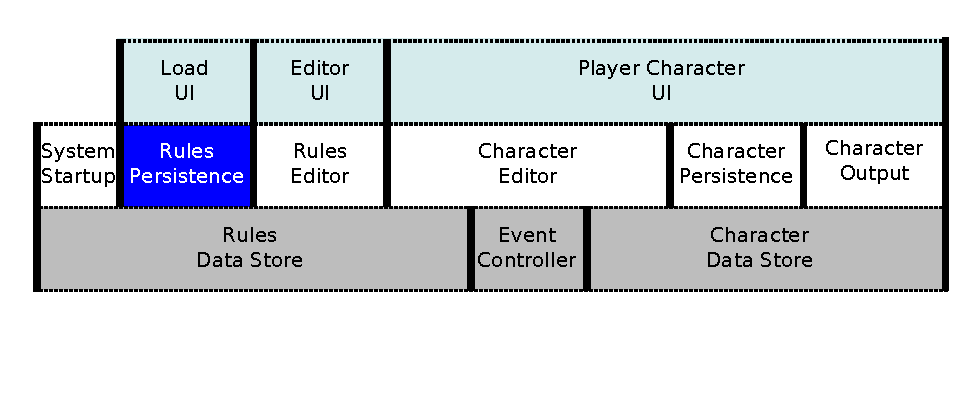
\includegraphics[width=6.5in]{rsf.pdf}}\closefig{\label{Fig: Layered Subsystems}Layered View of PCGen \pcgenvers subsystems}

\lnsection{Contributors}

Contributors to this document, either directly or by feedback and comments:\\
\contributors

\lsection{Document Conventions}

Java Classes, Interfaces, or other forms of items that can be found in the code are
presented in this document in \textem{italics}.  

\lnsection{\system - Background}

The \system is one of the major components of PCGen, and a focus area for PCGen \pcgenversEOS.

The \system is responsible for loading game system and component data from the
persistence data file format and saving it back into that data file format.  It is aware of the 
internal storage of information within PCGen only to the point it is required to store that
information for use by the core of PCGen.  The \system is not capable of interpreting much
in the way of meaning of the values it is storing.

This document describes the changes being implemented in the \systemEOS, and 
provides general guidance on how to interact with the interface/API of the \systemEOS.

\lsubsection{\system Major Concepts}

\lsubsubsection{The Data Persistence Format}

The data persistence format is typically known to the data developers as ``Game Mode'',
``PCC'' or ``LST'' files.  These vary slightly in syntax, but are generally tab-delimited
text files.  Generally ``PCC'' files are used to identify which ``LST'' files should be 
loaded, although there is also limited support for some Global tokens to be used in 
``PCC'' files.

\lsubsubsection{Data Load}

Load is the set of events that occurs when data persistence files are loaded into PCGen.
The Data Load process is intended to include full parsing of the data in the data 
persistence files (see \myref{Catch Errors Early}) and not while Player Characters are 
being created.  The Data Load process is shown in Figure \ref{Fig: Flow of Data Load}.

\lsubsubsection{Runtime}

Runtime processes and events are those that take place while a Player Character is 
being created.  The \system is not responsible for Runtime behavior, although the 
\system is responsible for ensuring that the Data Load process produces entries
in the Rules Data Store that minimizes the possible errors or unexpected conditions
at Runtime.

\lnsection{\system Sub-components}

\openfig\centerline{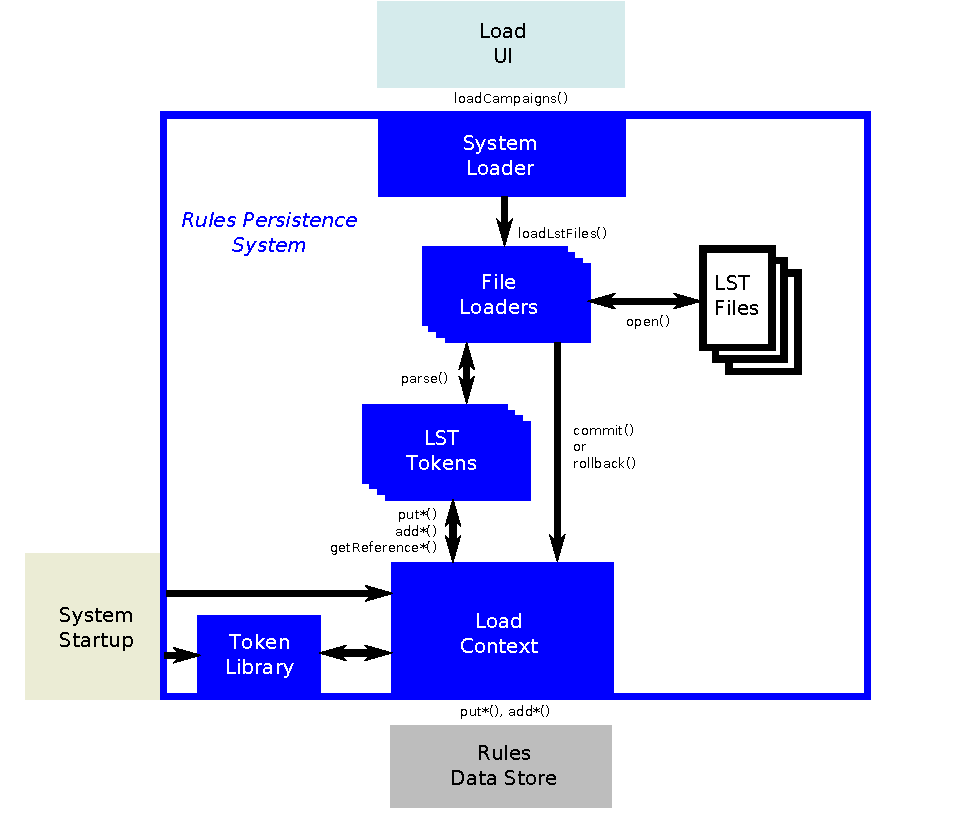
\includegraphics[width=6.5in]{rse.pdf}}\closefig{\label{Fig: Subcomponents and Relationships}View of PCGen \pcgenvers \system components and context to other subsystems of PCGen }

\openfig\centerline{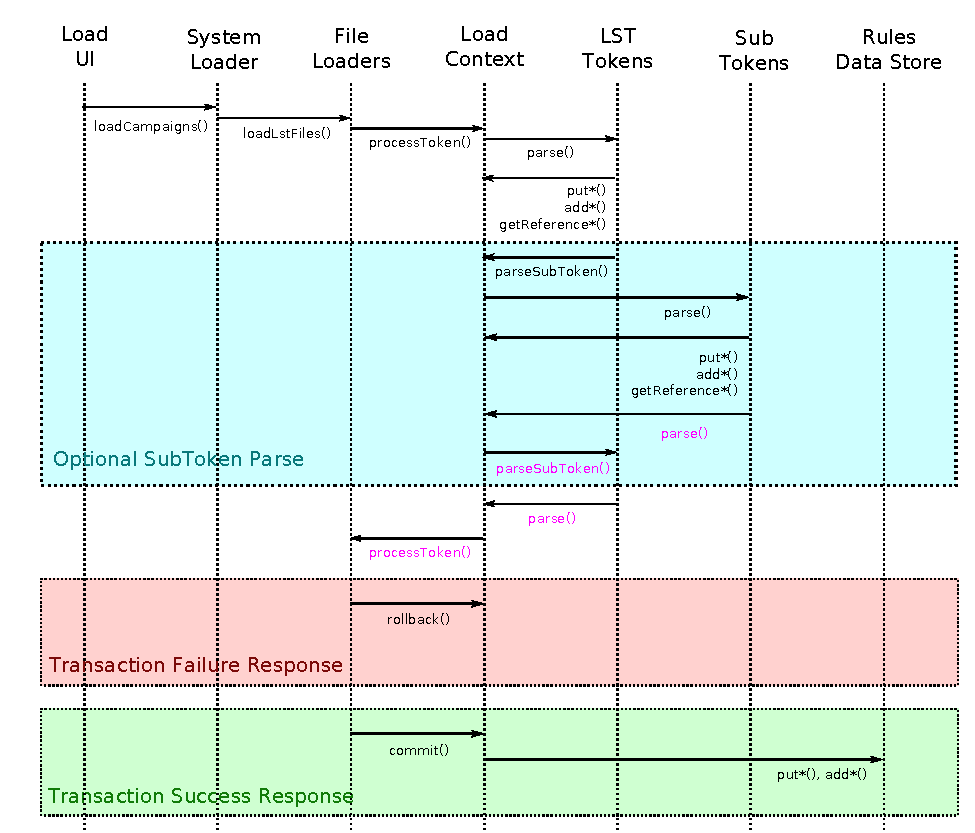
\includegraphics[width=6.5in]{rslf.pdf}}\closefig{\label{Fig: Flow of Data Load}Flow of Data Load in PCGen \pcgenvers \system }

\openfig\centerline{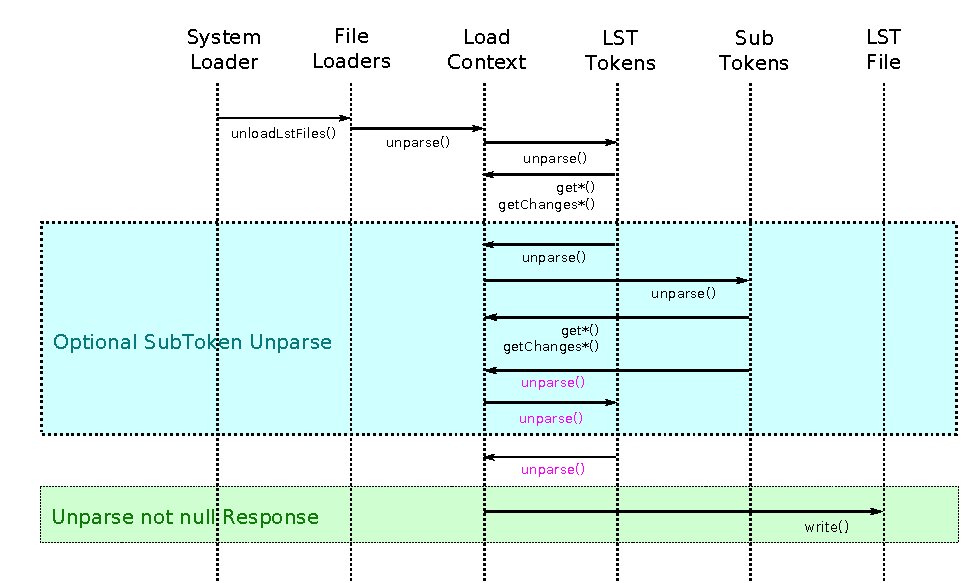
\includegraphics[width=6.5in]{rsuf.pdf}}\closefig{\label{Fig: Flow of Data Unload}Flow of Data Unload in PCGen \pcgenvers \system }

\lsubsection{System Loader}

The System Loader is responsible for receiving a set of Campaigns that should be 
loaded during Data Load.  These Campaigns are analyzed by the System Loader, and 
then the System Loader provides a list of Source Entries to each File Loader to
indicate what files (or more generally, URIs) should be loaded.

For backwards compatibility in the transition from PCGen 5.14, the System Loader is
in \textem{LstSystemLoader} in the \textem{pcgen.persistence.lst} package.

\lsubsection{File Loaders}

File Loaders are Classes that perform the specific actions necessary to load a specific 
LST file from the file system (or URI) and parse the file into
individual tags.  The File Loaders then identify the appropriate Token and pass the
value of the tag to the individual Token to be parsed.

For backwards compatibility in the transition from PCGen 5.14, the File Loaders are in the
\textem{pcgen.persistence} package.

\lsubsection{Tags and Tokens}

Data that defines the rule constructs of a Class, Race, Language, and other characteristics
and attributes of a PlayerCharacter are stored in LST files. These LST files are parsed to
import the information from those LST files into objects within the PCGen program. 

For purposes of this document, the individual entries in the data persistence
files will be referred to as ``Tags''. To store information, these tags separate the ``key''
(used to indicate the tag name) and the ``value'' (the information the tag is conveying to
PCGen) by a colon.  A simple example can be taken from the Common Language in the
Language LST file from SRD 3.0:\\
\texttt{TYPE:Spoken}

This indicates the ``TYPE'' tag is indicating a value of ``Spoken''.

For purposes of this document, the code that parses the value of a tag and translates the 
tag syntax into the internal data structure of PCGen is called a Token.

Occasionally, you fill find these the terms ``tag'' and ``token'' used differently;
which name is used will likely depend on the perspective of the
speaker.\footnote{This document makes effort to use the terms Tag and Token in the context
they are defined in this section.  This is a decision for clarity, and is not a judgement
of the ``best'' method for referring to the items in the data persistence format or the code.}

Types of tokens for PCGen \pcgenvers are located in \textem{pcgen.rules.persistence.token}.  
Table \ref{Token Interfaces} explains the different types of tokens, in order
to clarify the use of each of the token interfaces.

\begin{table}
\begin{center}
\begin{tabular}{ | m{2.1in} | m{4in} | }
\hline
  \textbf{Token Interface from \textem{pcgen.rules.persistence.token}} & \textbf{Interface Description} \\  \hline \hline
  CDOMToken & A \textem{CDOMToken} is a PCGen \pcgenvers token that has a \textem{parse()} method for processing the value of a tag and a \textem{getTokenName()} method  to identify the name of the tag the Token can process.  Note that a \textem{CDOMToken} does not require \textem{unparse()}, as compatibility tokens from previous revisions would not implement that behavior. \\ \hline
  CDOMPrimaryToken & A \textem{CDOMPrimaryToken} is a \textem{CDOMToken} that is active (not deprecated) in the current version of PCGen, and thus implements the \textem{unparse()} method. \\ \hline
  CDOMSubToken & A \textem{CDOMSubToken} is a \textem{CDOMToken} that is designed to operate for subtokens (see \myref{Subtokens}). \\ \hline
  CDOMSecondaryToken & A \textem{CDOMSecondaryToken} is a \textem{CDOMSubToken} that is active (not deprecated) in the current version of PCGen, and thus implements the \textem{unparse()} method. \\ \hline
  CDOMCompatibilityToken & A \textem{CDOMCompatibilityToken} is a \textem{CDOMToken} that implements a tag syntax from a previous version of PCGen, see \myref{Token Compatibility}. Once deprecated, a \textem{CDOMPrimaryToken} would become a \textem{CDOMCompatibilityToken}. \\ \hline
  CDOMCompatibilitySubToken & A \textem{CDOMCompatibilitySubToken} is a CDOMSubToken that implements a tag syntax from a previous version of PCGen, see \myref{Token Compatibility}. Once deprecated, a \textem{CDOMSecondaryToken} would become a \textem{CDOMCompatibilitySubToken}. \\ \hline
  ClassWrappedToken & A \textem{ClassWrappedToken} is a specialized \textem{CDOMToken} designed to provide compatibility for using CLASS tokens on the level 1 CLASSLEVEL line, see \myref{Class Wrapped Token}. \\ \hline
  PreCompatibilityToken & A \textem{PreCompatibilityToken} is a token for wrapping the PCGen 5.14-type Prerequisite tokens into \pcgenversEOS-type tokens, see \myref{Prerequisite Tags}. \\ \hline
\end{tabular}
\end{center}
\caption{Token Interfaces and usage in PCGen \pcgenvers}
\label{Token Interfaces}
\end{table}

Tokens that implement these interfaces, which are effectively extensions to the \systemEOS,
are found in the \textem{plugin.lsttokens} package.

\sbnote{A Note of Caution on Tags/Tokens}{Different tags have different behavior with respect to 
overwriting or appending values.  Some tags may only allow a single value (e.g. RACETYPE
from Race LST files), and subsequent references to that tag in the same object
will overwrite the original value. Other tags are effectively lists
(e.g. the Global TYPE tag), and subsequent calls to that tag
will append values to the list.  The behavior should be noted within the tag documentation
distributed with PCGen.}

\lsubsection{Load Context}

The Load Context represents the translator of information loaded in
File Loaders and Tokens.  The translation is from the persistence data file format 
to the internal structure used by the Rules Data Store.  The LoadContext provides
various services; some are discussed in later sections.

Context Classes of the \system are found in the \textem{pcgen.rules} package.

\lsubsection{Token Library}

The Token Library is the storage location for the Tokens, and is queried by the LoadContext
once the key and value of a tag has been established by a File Loader.  The Token Library is
initialized by the Startup System when plugins are loaded by PCGen.

\lnsection{Functional Requirements}

The following functional requirements are provided for use in understanding the basis for the PCGen \pcgenvers
\system architecture. Functional requirements are constraints on features as they appear to a user
of PCGen \pcgenversEOS.  Many of these Functional Requirements are shared with the overall PCGen 
Functional Requirements.

\lsubsection{Compatibility with Previous Versions}

PCGen \pcgenvers must be capable of fully loading PCGen 5.14 LST data files.  Data from older 5.x releases
(in particular PCGen 5.12 and 5.10) may be compatible with PCGen \pcgenversEOS; however, there are known
ambiguities that prevent 100\% compatibility with older releases.  

This requirement must be met.  Other features of the system (requirements and other good design guidelines)
will be sacrificed to meet this requirement.

\basis There is a tremendous investment in the PCGen 5.x code, data and documentation.  This compatibility
requirement ensures the ability to leverage that time investment, especially in data and documentation.

\lsubsection{Increased Flexibility}

Eliminating hard coded values and special cases that currently exist in the PCGen code base will
allow PCGen to more easily support non-d20 systems.  In addition, increased flexibility will provide
for faster feature enhancement, providing additional benefit to users.

\basis Desire for faster turnover of feature requests, and long-term strategy to expand 
the PCGen universe to include non-d20 based game systems to increase function
for existing users and to attract new users to PCGen.

\lnsection{Structural Requirements}

The following structural requirements are provided for use in understanding the basis for the
PCGen \pcgenvers \system architecture.  Structural requirements are constraints on features as they appear
to a developer of PCGen \pcgenversEOS.\footnote{It is recognized that some of these items would
qualify more as ``design'' than ``architecture'', as they are general features or characteristics
of well-written software systems.  Without any disrespect for software architecture purists, we
include a number of those design characteristics, as they help to contrast the PCGen 
\pcgenvers architecture from architecture of earlier versions of PCGen.}   Many of these Structural
Requirements are shared with the overall PCGen Structural Requirements.

\lsubsection{Minimize Process/Structural Models}

PCGen \pcgenvers \system should have a minimal set of design structures used to specify the functions
required to build a Player Character. 

\basis This minimizes the number of mental models a developer must understand. Reduced quantity
of design patterns and structures improves the ability of new (and existing!) developers to
understand the code.  This also allows greater code reuse and reduces code duplication (which
is subject to copy/paste error).  Selection of appropriate models will also reduce the number
of exceptions in the code, eliminating further risk of bugs and confusion for developers.

\lsubsection{Information Hiding}

The format of data files on disk should be independent of the processing of a game system or
Player Character

\basis This insulates the code (modifying a player character or the game system data)
from changes in the data file format.  This increases the flexibility to add features to
PCGen without core changes.  This facilitates unit testing by improving component isolation.

\lsubsection{Data Encapsulation}

There should be defined and limited interfaces between modules of PCGen.

\basis This improves code maintainability.  This truly insulates modules of PCGen from
changes elsewhere in the system.  This therefore facilitates parallel development.  This
also improves the ability to unit test the code, as ``mock'' objects that implement the
framework can be used for testing.

\lsubsection{Catch Errors Early}

Errors in the data files should be caught during data persistence file load, and should not
trigger runtime errors.
 
\basis Given the \system being independent of the internal data structure,
all items will be resolved at Data Load.  This will ensure that all objects
in a given namespace possess a unique KEY, regardless of the source file.  In addition,
all object references can be validated to ensure an object that was actually
constructed and loaded.

\lsubsection{Stable Code Structure}

Dependency between packages and classes will result in a Directed Acyclic Graph.

\basis The PCGen code base is over 2,000 classes.  This is a significant code base and
requires isoloating subsystems and defining dependencies in order to minimize the impact
of code changes.  Improved code structure also facilitates testing.  Eliminating tangles
in Class dependency will improve the ability to write true unit tests (tests that work on a
single Class).  This means it will be possible to catch smaller errors due to incorrect
modifications of the PCGen code base.  Improved structure also facilitates understanding
of the code by developers.  The overall impact of good code structure is seen to both
developers and end users as improved speed and ability to modify the PCGen code.

\lsubsection{Avoid Contracts}

Two forms of contracts should be avoided: (1) When a developer makes a code modification,
the developer should not be forced to make a matching modification in another location in the
code. (2) When a change is made to the internal data structure, a significant amount of
``reorganization'' to ensure a valid data structure should not be necessary.

\basis Contracts cause problems because they introduce bugs into software when matching changes
are not made.  They also make it more difficult for developers to understand the architecture
of a system, because they are forced to focus on adhering to the contracts.  Data structure
contracts can result in invalid data structures, and often lead to performance issues as the
data structure is validated and corrected.

\lsubsection{Minimize Order Dependency}

The number of order dependent operations should be minimized.

\basis Order dependency can cause significant issues, especially as it is hard to maintain
accurate documentation of such restrictions.  Operations that are not order dependent can
also be parallelized (e.g. on multi-processor systems) to improve performance.

\lnsection{\system Key Design Decisions}

\lsubsection{Token/File Loader System}

This is a shared design characteristic with PCGen 5.14.  File Loaders are key components of
the \systemEOS.  File Loader instances are specific to a given file type.  When processing
a file, the File Loader splits the file into separate lines, splits the lines (if necessary)
into separate tags, and then submits the tags to the Tokens.

\under \myref{Information Hiding}, \myref{Data Encapsulation}, \myref{Increased Flexibility}

\basis This abstracts specific individual components of the data persistence format from the
internal data structure (and each other).

\impl The interactions of Tokens, File Loaders and other elements of the \system is shown in
Figure \ref{Fig: Flow of Data Load}.

File Loaders are created by the \system for each file type.  While these may share 
a single Class (for code reuse), each instance is specialized to a specific data persistence
format file type.  The list of available tags is also specific to a given data persistence
file type.  This allows features to be limited to certain objects to avoid non-sensical
situations (e.g. you can't assign types of material components to a Race).  A collection
of Global tags that can be used in nearly all data persistence files is also available.

Each Token Class is stored in a separate file, independent of the core of PCGen, to allow each 
token to be independently updated, removed, or otherwise manipulated without altering or
impacting other Tokens.  Individual Token files are in the \textem{pcgen.plugin.lsttokens} package. 
These persistence Tokens are non-abstract Classes that
implement the \textem{LstToken} interface.  When PCGen is launched, all plugins of PCGen are 
evaluated, and Tokens are specifically placed into the \textem{TokenLibrary}.  The Tokens each
have a method (\textem{getTokenName()}) that identifies the tag the Token processes.

By keeping each Token in an individual class, this keeps the Token Classes very simple,
which makes them easy to test, modify, and understand (as they are effectively atomic to the
processing of a specific token).  One goal of the PCGen \system is to ensure that all of the
parsing of LST files is done within the Tokens and not in the core of PCGen.  This makes
adding new tags to the LST files to be reasonably painless (though changes to the core or
export system may also be required to add required functionality).   It at least facilitates
the long-term goal of altering behavior of PCGen without forcing a recompile of core PCGen
code.

\sbnote{On Transition from PCGen 5.14}{PCGen 5.14 used a slightly different storage system
for tokens.  It stored tokens in a \textem{TokenStore}, and that was effectively done under 
a Map of Maps.  The first Map was an interface identifying the type of Token, and the second 
Map was used to identify the token from the tag name.  As the conversion to the new Token
system is being done gradually, some tokens in PCGen \pcgenvers may remain in the PCeGen 5.14 
style.  New tokens will always extend (perhaps indirectly through another Interface),
\textem{CDOMToken}.}

\lsubsection{Data Modification during Data Load}

This is a shared design characteristic with PCGen 5.14.  The \system supports
modifying, copying or forgetting objects defined in the data persistence files.

\under \myref{Information Hiding}, \myref{Data Encapsulation}, \myref{Increased Flexibility}

\basis This allows users to modify base data to easily produce new Races, Abilities, or other items
without risk of copy/paste error.

\impl The data persistence file format supports three special functions that can be performed
on data persistence entries.

\begin{description}
\item[.COPY] allows a data file to copy an existing object. This .COPY entry need not worry about
file load order (see \myref{Data Persistence File Load Order Independence}).  The value preceding
the .COPY string identifies the object to be copied.  This identifier is the KEY
(or KEY and CATEGORY) of the object to be copied.  The identifier for the copied object is placed 
after an equals sign that follows the .COPY String, e.g.:\\
\texttt{Dodge.COPY=MyDodge}
\item[.MOD] allows a data file to modify an existing object.  This .MOD entry need not worry about
file load order (see \myref{Data Persistence File Load Order Independence}).  All .MOD entries will
be processed after all .COPY entries, regardless of the source file.  The value preceding
the .MOD string identifies the object to be modified.  This identifier is the KEY
(or KEY and CATEGORY) of the object to be modified.  If more than one .COPY token produces an 
object with the same identifier, then a duplicate object error will be generated.
\item[.FORGET] allows a data file to remove an existing object from the Rules Data Store.  This 
.FORGET entry need not worry about file load order
(see \myref{Data Persistence File Load Order Independence}).  All .FORGET entries will
be processed after all .COPY and .MOD entries, regardless of the source file.  The value preceding
the .FORGET string identifies the object to be removed from the Rules Data Store.  
\end{description}

\lsubsection{Subtokens}

This is a shared design characteristic with PCGen 5.14.  Some tags have complex behavior
that significantly differs based on the first argument in the value of the tag.  In order
to simplify tag parsing and Token code, these Tokens implement a Sub-token structure, 
which delegates parsing of the tag value to a Token specialized to the first argument
in the value of the tag.

\under \myref{Data Encapsulation}, \myref{Information Hiding}, \myref{Increased Flexibility}

\basis This design is primarily intended to separate out code for different subtokens.  This
provides increased ability to add new subtokens without altering existing code.  This provides
increased flexibility for developers, and ensures that unexpected side effects from code changes
don't impact other features of PCGen.

\impl The flow of events during Data Load when Subtokens are present is shown as an optional
series of events in Figure \ref{Fig: Flow of Data Load}.

The LoadContext is capable of processing subtokens for a given Token.  Any token 
which delegates to subtokens can call \textem{processSubToken(T, String, String, String)}
from LoadContext in order to delegate to subtokens.  This delegation will return a boolean 
value to indicate success (\textem{true}) or failure (\textem{false}) of the delegation. 
The exact cause of the failure is reported to the \textem{Logging} utility.

Note that it is legal for a subtoken to only be valid in a single object type (such as
a Race), even if the ``primary'' token is accepted universally.  This greatly simplifies 
the restriction of subtokens to individual file types without producing burden on
the primary token to establish legal values.  Resolution of those restrictions is handled
entirely within the LoadContext.

\lsubsection{\system I/O}

The input and output of data persistence information should be an integral part of the
\systemEOS.  In PCGen 5.14, Tokens and the \system were only responsible for input from 
the data persistence file format.  In PCGen \pcgenversEOS, the \system is responsible
for both input and output.

\under \myref{Data Encapsulation}, \myref{Information Hiding}

\basis Adding output to the persistence system provides the ability to reuse the 
\system in a data file editor, as well as the runtime system.  This sharing
of code helps to guarantee the integrity of the data file editor.  Such a structure
also facilitates unit testing, as the \system can be tested independently
of the core code.

\impl Each token has the ability to both ``parse'' and ``unparse'' information 
for the \systemEOS.  Parsing is the act of reading a token value from a data 
persistence file and placing it into the internal rules data structure.  Unparsing
is the act of reading the internal data structure and writing out the appropriate
syntax into a data persistence file.

In addition to other benefits, this parse/unparse structure allows Tokens to be
tested without major dependence on other components of PCGen.  These tests are found in 
\textem{plugin.lsttokens package} of the \textem{code/src/utest} source directory.

As explained in Section \ref{Token/File Loader System}, Token/File Loader System, the File Loaders
separate out the tags in an input file and call the parse method on the appropriate
Tokens.  In order to unparse a loaded object back to the data persistence syntax, the 
all Tokens that could be used in the given object type must be called.

Unparsing a particular object is managed by the \textem{unparse(T)}
method of \textem{LoadContext}.  This process includes delegation of the unparse to all
subtokens (See section \ref{Subtokens}), as depcited in Figure \ref{Fig: Flow of Data Unload}. 

Because all tokens are called when unparsing an object, it is important that tokens 
properly represent when they are not used.  This is done by returning \textem{null} from
the \textem{unparse} method of the Token.  

Some tokens can be used more than once in a given object (e.g. BONUS), and thus must be 
capable of indicating each of the values for the multiple tag instances.  Since Tokens 
do not maintain state, the unparse method must only be called a single time to get all
of the values; thus, the unparse method returns an array of String objects to indicate 
the list of values for each instance of the tag being unparsed.

The context is responsible for loading the returned value with the name of the tag; 
just as the token is not responsible for removing/ignoring the name of the tag in
the value passed into the \textem{parse} method, it does not prepend the name of the tag
to the value(s) returned from the \textem{unparse} method.

\lsubsection{Independent Data Persistence Interface}

The Data Persistence format must be independent of internal data structure. (The subsystems of PCGen 
other than the \system should not have detailed knowledge of the data persistence file format).

\under \myref{Information Hiding}, \myref{Catch Errors Early}

\basis This abstracts the data persistence format from the internal data structure.  It forces the entire
persistence contents to be parsed on data load.  This ensures any errors in data files are
caught in the \system at data load, rather than at runtime.

\impl During the load of data from the data persistence format, each Token is required to 
fully parse the information and validate the information as much as possible.  This ensures 
that errors in the data files are caught as they are loaded, and not at runtime.  The \system
is responsible for ensuring data integrity of the rules data to the rest of the PCGen system, 
and the Tokens are the ``front lines'' of fulfilling that responsibility.

Beyond the tokens, a load subsystem translates between the data persistence file format parsed by 
the Tokens and the internal data structure.\footnote{Some might argue this
system fits the Data Mapper design pattern, although it's not strictly using relational databases.}
This system is currently known as a \textem{LoadContext}.  The details of translation takes
various forms, and those structures are explained in later sections.

\lsubsection{Only valid Tokens may impact the Rules Data Store}

There is a risk that a partially-parsed Token from an invalid data persistence entry could
lead to an unknown state within the Rules Data Store.  Therefore, a Token should only be
responsible for controlling the state of the Rules Data Store if the token parse
completes successfully.

\under \myref{Information Hiding}

\basis This greatly simplifies the implementation of Tokens, as they are not required to
analyze or defer method calls to the \textem{LoadContext} until after the data persistence syntax
is established to be valid.

\impl During the load of data from the data persistence format, each Token may fully parse
the provided value and make any necessary calls to the LoadContext.  This can be done even if
subsequent information indicates to the Token that there is an error in the Token value.  
Specifically, individual Tokens should be free to take any action on the \textem{LoadContext}, 
and are not responsible for the consequences of those method calls unless the Token indicates
that the value from the data persistence format was indicated to be valid.  This indication of 
validity is by returning \textem{true} from the parse method of the Token.\footnote{This is 
effectively the \textem{Unit of Work} design pattern}

If a Token returns \textem{true}, indicating the token was valid, then the File Loader that
called the Token is responsible for indicating to the \textem{LoadContext} to \textem{commit()}
the changes defined by the Token.  This proces is shown in the ``Transaction Success Response''
section in Figure \ref{Fig: Flow of Data Load}.

If the Token returns \textem{false}, then the File Loader is
responsible for calling the \textem{rollback()} method of \textem{LoadContext} to indicate
no changes should made to the Rules Data Store and the tentative changes proposed by the Token
should be discarded.  This proces is shown in the ``Transaction Failure Response'' section
in Figure \ref{Fig: Flow of Data Load}.

\lsubsection{Data Persistence File Load Order Independence}

Items in the rules structure may refer to each other, by granting certain features, possessing
certain prerequisites, or by other means.  For example, an Ability A may grant Ability B, but
we cannot reasonably require that Ability A appears before Ability B.  More specifically, due
to known interactions, it is impossible to choose a load order for files and entries 
that guarantees objects will be constructed before references to those objects
are encountered.  Order independence of persistent data is therefore an architectural requirement.

\under \myref{Information Hiding}, \myref{Data Encapsulation}, \myref{Catch Errors Early}

\basis Using references before objects are constructed to ensure full parsing of the data
persistence file syntax during load improves error catching capability at load time and 
should improve runtime performance.  

\impl A two pass load system is required in order to ensure separation of the data
persistence format and the internal data structure.  In
PCGen \pcgenvers, any Token may request a reference to an object, regardless of whether that object has 
been constructed in the \textem{LoadContext}.  This is done through a \textem{ReferenceContext}.
The \textem{ReferenceContext} is capable of returning three types of references.  

\begin{description}
\item[Single References] refer to a single object, and are useful in situations where single elements (or 
perhaps lists of single elements) are specified in the value of the Token.  
\item[Type References] refer to groups of objects, and are used in situations where entire types are
referenced by the TYPE= identifier.
\item[All References] refer to all objects of a given type, and are used in situations where the
special "ALL" or "ANY" identifiers are used.
\end{description}

These references requested by the tokens can then be placed into objects (Abilities, Skills, etc.)
and the underlying object(s) to which the reference refers can be established at runtime.

There are two issues introduced with a system that is capable of referencing objects before
they are constructed.  

The first issue is that references might be made to objects that don't exist.  This problem 
cannot be detected until the entire load operation is complete.  The \system makes a call to
the \textem{validate()} method of \textem{ReferenceContext} to test whether any references were
made where the appropriate referred-to object was not constructed during data persistence file load.
In order to provide for minimal functionality without truly understanding the reference, PCGen 
\pcgenvers constructs a dummy (empty) object with the given identifier.

Second, the References constructed during data persistence file load
must be resolved before they are used during ``runtime''.  Therefore, the
\system is responsible for resolving any references after a collection of Campaigns are loaded.
This resolution is driven through the \textem{resolveReferences()} method of \textem{LoadContext}.
Due to the construction of dummy objects during the \textem{validate()} step,
\textem{resolveReferences()} must be called after \textem{validate()}.

\lsubsection{Shared Persistence System with Editor}

The data persistence system should be usable for both a data file editor and the
runtime character generation program.

\under Code Reuse (general design characteristic), \myref{Catch Errors Early}

\basis A significant investment made in ensuring that persistent data is read
without errors should be reused across both a data file editor and the runtime
system.  Consolidation reduces the risk of error and ensures that the editor
will always be up to date (a problem in PCGen 5.14).  In addition, additional
editing capabilities (e.g. edit data in place) that are not available in PCGen
5.14 can be added once a full-capability editor is available.

\impl The \system is responsible for tracking detailed changes made by the Tokens during 
Data Load (see \myref{Only valid Tokens may impact the Rules Data Store}).  As a result,
this information allows the load system to serve as a runtime load system and a 
file editor load system.

As noted in \myref{\system I/O}, tags may overwrite previous values
or add to the set of values for that tag.  In the case of an editor,
it is critically important not to lose information that
would later be overwritten in a runtime environment.  A simple example would be 
the use of a .MOD to alter the number of HANDS on a Race.  This alteration should
be maintained in the file that contained the .MOD and the value (or unspecificied
default) in the original Race should not be lost.  This is done by tracking the
URI from which data is loaded.

In order to maintain simplicity in the Tokens, they are kept URI-ignorant.  File Loaders
are responsible for calling the \textem{setSourceURI(URI)} method on LoadContext
to identify the source of data being processed in the \textem{parse()} method of a Token.
File Loaders are also responsible for calling the \textem{setExtractURI(URI)} method
on LoadContext to identify any restriction on data that should be written out
during calls to the \textem{unparse()} method of a Token.  The LoadContext is responsible
for restricting responses to the extract URI in return values from any methods used by
\textem{unparse()} to extract information from the LoadContext.

\lsubsection{Token Compatibility}

***PLACEHOLDER: Describe Compatibility system and impact on TokenLibrary***

\lnsection{Known Issues}

\lsubsection{Prerequisite Tags}

Currently the Prerequisite tags are an exception to the parsing system.  The Prerequisite tags
have a prefix of "PRE" and are followed by the Prerequisite name, e.g. PREFEAT.  This means that 
the Prerequisite tags do not follow the traditional method of having a unique name before 
the colon.  Also, Prerequisite tags can have a leading ! to negate the Prerequisite.

In order to address this situation of a different token definition system, the
\textem{PreComatibilityToken} provides a wrapper into the new PCGen \pcgenvers token syntax. 

There is a feature request to convert the Prerequisite tags into two separate buckets, PRE: and REQ: 
(Prerequisites and Requirements) based on their current behavior.  This is (probably) not within
the scope of PCGen \pcgenversEOS. 

\lsubsection{Class Wrapped Token}

The point behind a ClassWrappedToken is to provide compatibility for what may be bad
behavior in data files.

Many Class tokens in PCGen 5.14 ignore the class level, so they are technically Class tags
and not CLASSLEVEL tags. Yet, PCGen 5.14 allows those tags to
appear on class level lines.  This is a bit deceptive to users in that the effect will always
be on the class, and not appear on the specified level.

Unfortunately, one cannot simply remove support for using CLASS tokens on CLASSLEVEL lines, 
because if they are used at level 1, then they are equivalent to appearing on a CLASS line.  
Certainly, the data monkeys use it that way.  For example, Blackguard in RSRD advanced uses
EXCHANGELEVEL on the first level line.

Therefore the entire ClassWrappedToken system is a workaround for data monkeys using CLASS
tokens on CLASSLEVEL lines, and therefore it should only work on level one, otherwise
expectations for when the token will take effect are not set.

%\newpage
%\printindex

\end{document}

